%!TEX root = ../template.tex
%%%%%%%%%%%%%%%%%%%%%%%%%%%%%%%%%%%%%%%%%%%%%%%%%%%%%%%%%%%%%%%%%%%%
%% chapter4.tex
%% NOVA thesis document file
%%
%% Chapter with lots of dummy text
%%%%%%%%%%%%%%%%%%%%%%%%%%%%%%%%%%%%%%%%%%%%%%%%%%%%%%%%%%%%%%%%%%%%

\typeout{NT FILE chapter4.tex}%

\chapter{Implementation}
\label{cha:implementation}

In this chapter, we present the implementation of our system and discuss alternatives to the decisions we took in our implementation.
A modular approach was adopted to construct the system;
each module is entirely independent, making it easy to interchange alternative approaches.
We dedicate the first half of this chapter to define the goals that guided the design of system,
the remainder of the chapter will be used to discuss each design aspect in turn.

\section{Architecture} % (fold)
\label{sec:architecture}

\begin{figure}[htbp]
    \centering
    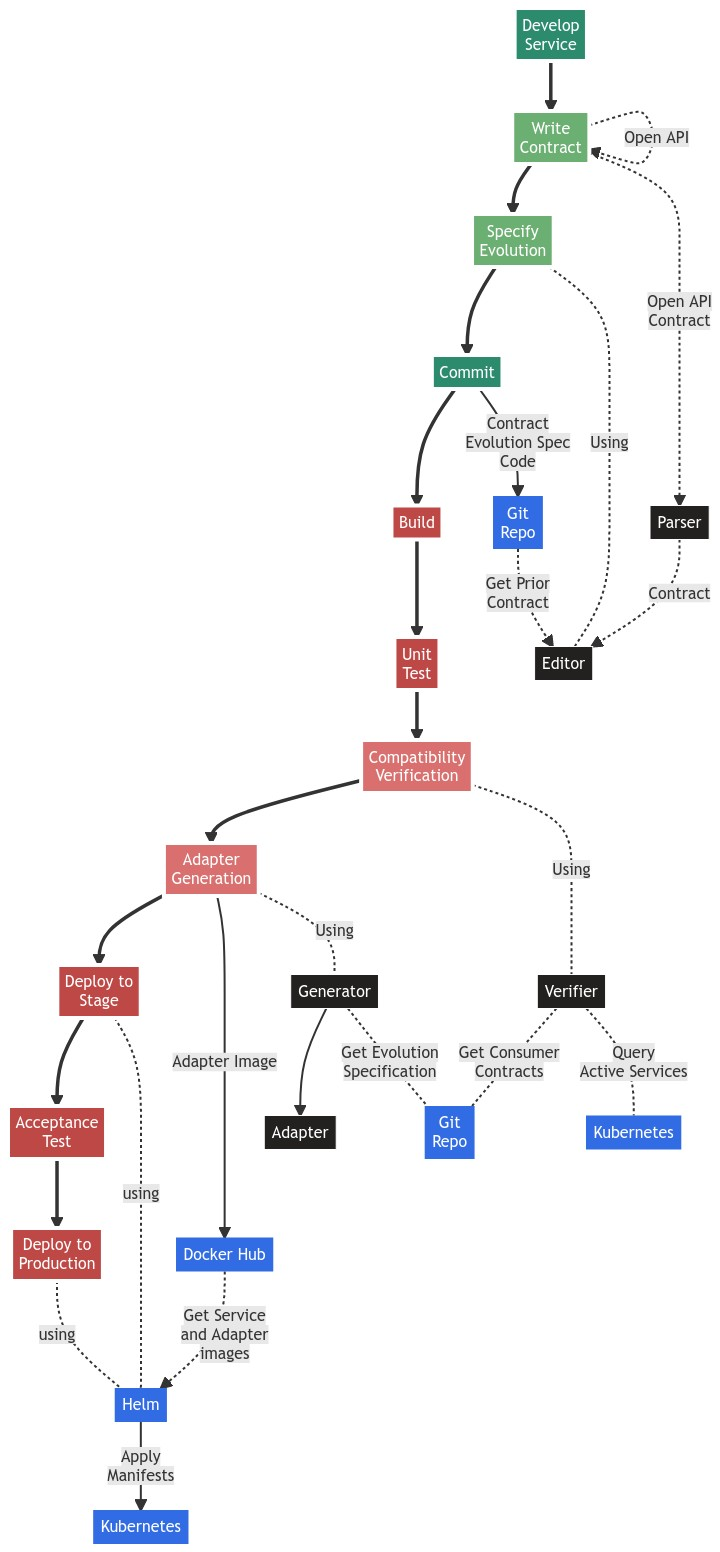
\includegraphics[height=9in]{architecture}
    \label{fig:gantt}
\end{figure}

\section{Parser} % (fold)
\label{sec:parser}

\paragraph{Description}
\paragraph{Capabilities}
An HTTP contract contains the HTTP method, the
path, the parameter schema, and the location of parameters (path, query, header); the
proposed compatibility verification approaches supports all of these elements.
\paragraph{Limitations}
\paragraph{Dependencies}

\section{Editor} % (fold)
\label{sec:editor}

\paragraph{Description}
\paragraph{Capabilities}
\paragraph{Limitations}
\paragraph{Dependencies}

\section{Verifier} % (fold)
\label{sec:verifier}

\paragraph{Description}
\paragraph{Capabilities}
\paragraph{Limitations}
\paragraph{Dependencies}

\section{Generator} % (fold)
\label{sec:generator}

\paragraph{Description}
\paragraph{Capabilities}
\paragraph{Limitations}
\paragraph{Dependencies}

\section{Adapter} % (fold)
\label{sec:adapter}

\paragraph{Tuning}. The demo application image was built using Ubuntu 18.04.6 as a base image and consists of Spring-boot microservice with a Apache Tomcat/9.0.65 http server.
In order to prevent the JVM from resizing and reallocating the heap memory while Tomcat is trying to serve requests and
calling garbage collector frequently, the JVM has started with a higher heap memory maximum, and the initial heap memory
size was set to the same value as its maximum memory size.
The maximum number of threads for Tomcat was set to 2000, in order to support a higher load of requests.

\paragraph{Description}
\paragraph{Capabilities}
\paragraph{Limitations}
\paragraph{Dependencies}

\section{Registry} % (fold)
\label{sec:registry}

\paragraph{Description}
\paragraph{Capabilities}
\paragraph{Limitations}
\paragraph{Dependencies}
